\chapter{Supplemental Material for Chapter \ref{chap:chapter 3}}

%%%%%%%%%%%%%%%%%%%%%%%%%%%%%%%%%%%%%%%%%%%%%%%%%%%%%%%%%%%%%%%%%%%%%%%%%%%%%%%%
\section{Supplementary Figures}
%%%%%%%%%%%%%%%%%%%%%%%%%%%%%%%%%%%%%%%%%%%%%%%%%%%%%%%%%%%%%%%%%%%%%%%%%%%%%%%%

\begin{figure}[p]
    \centering
    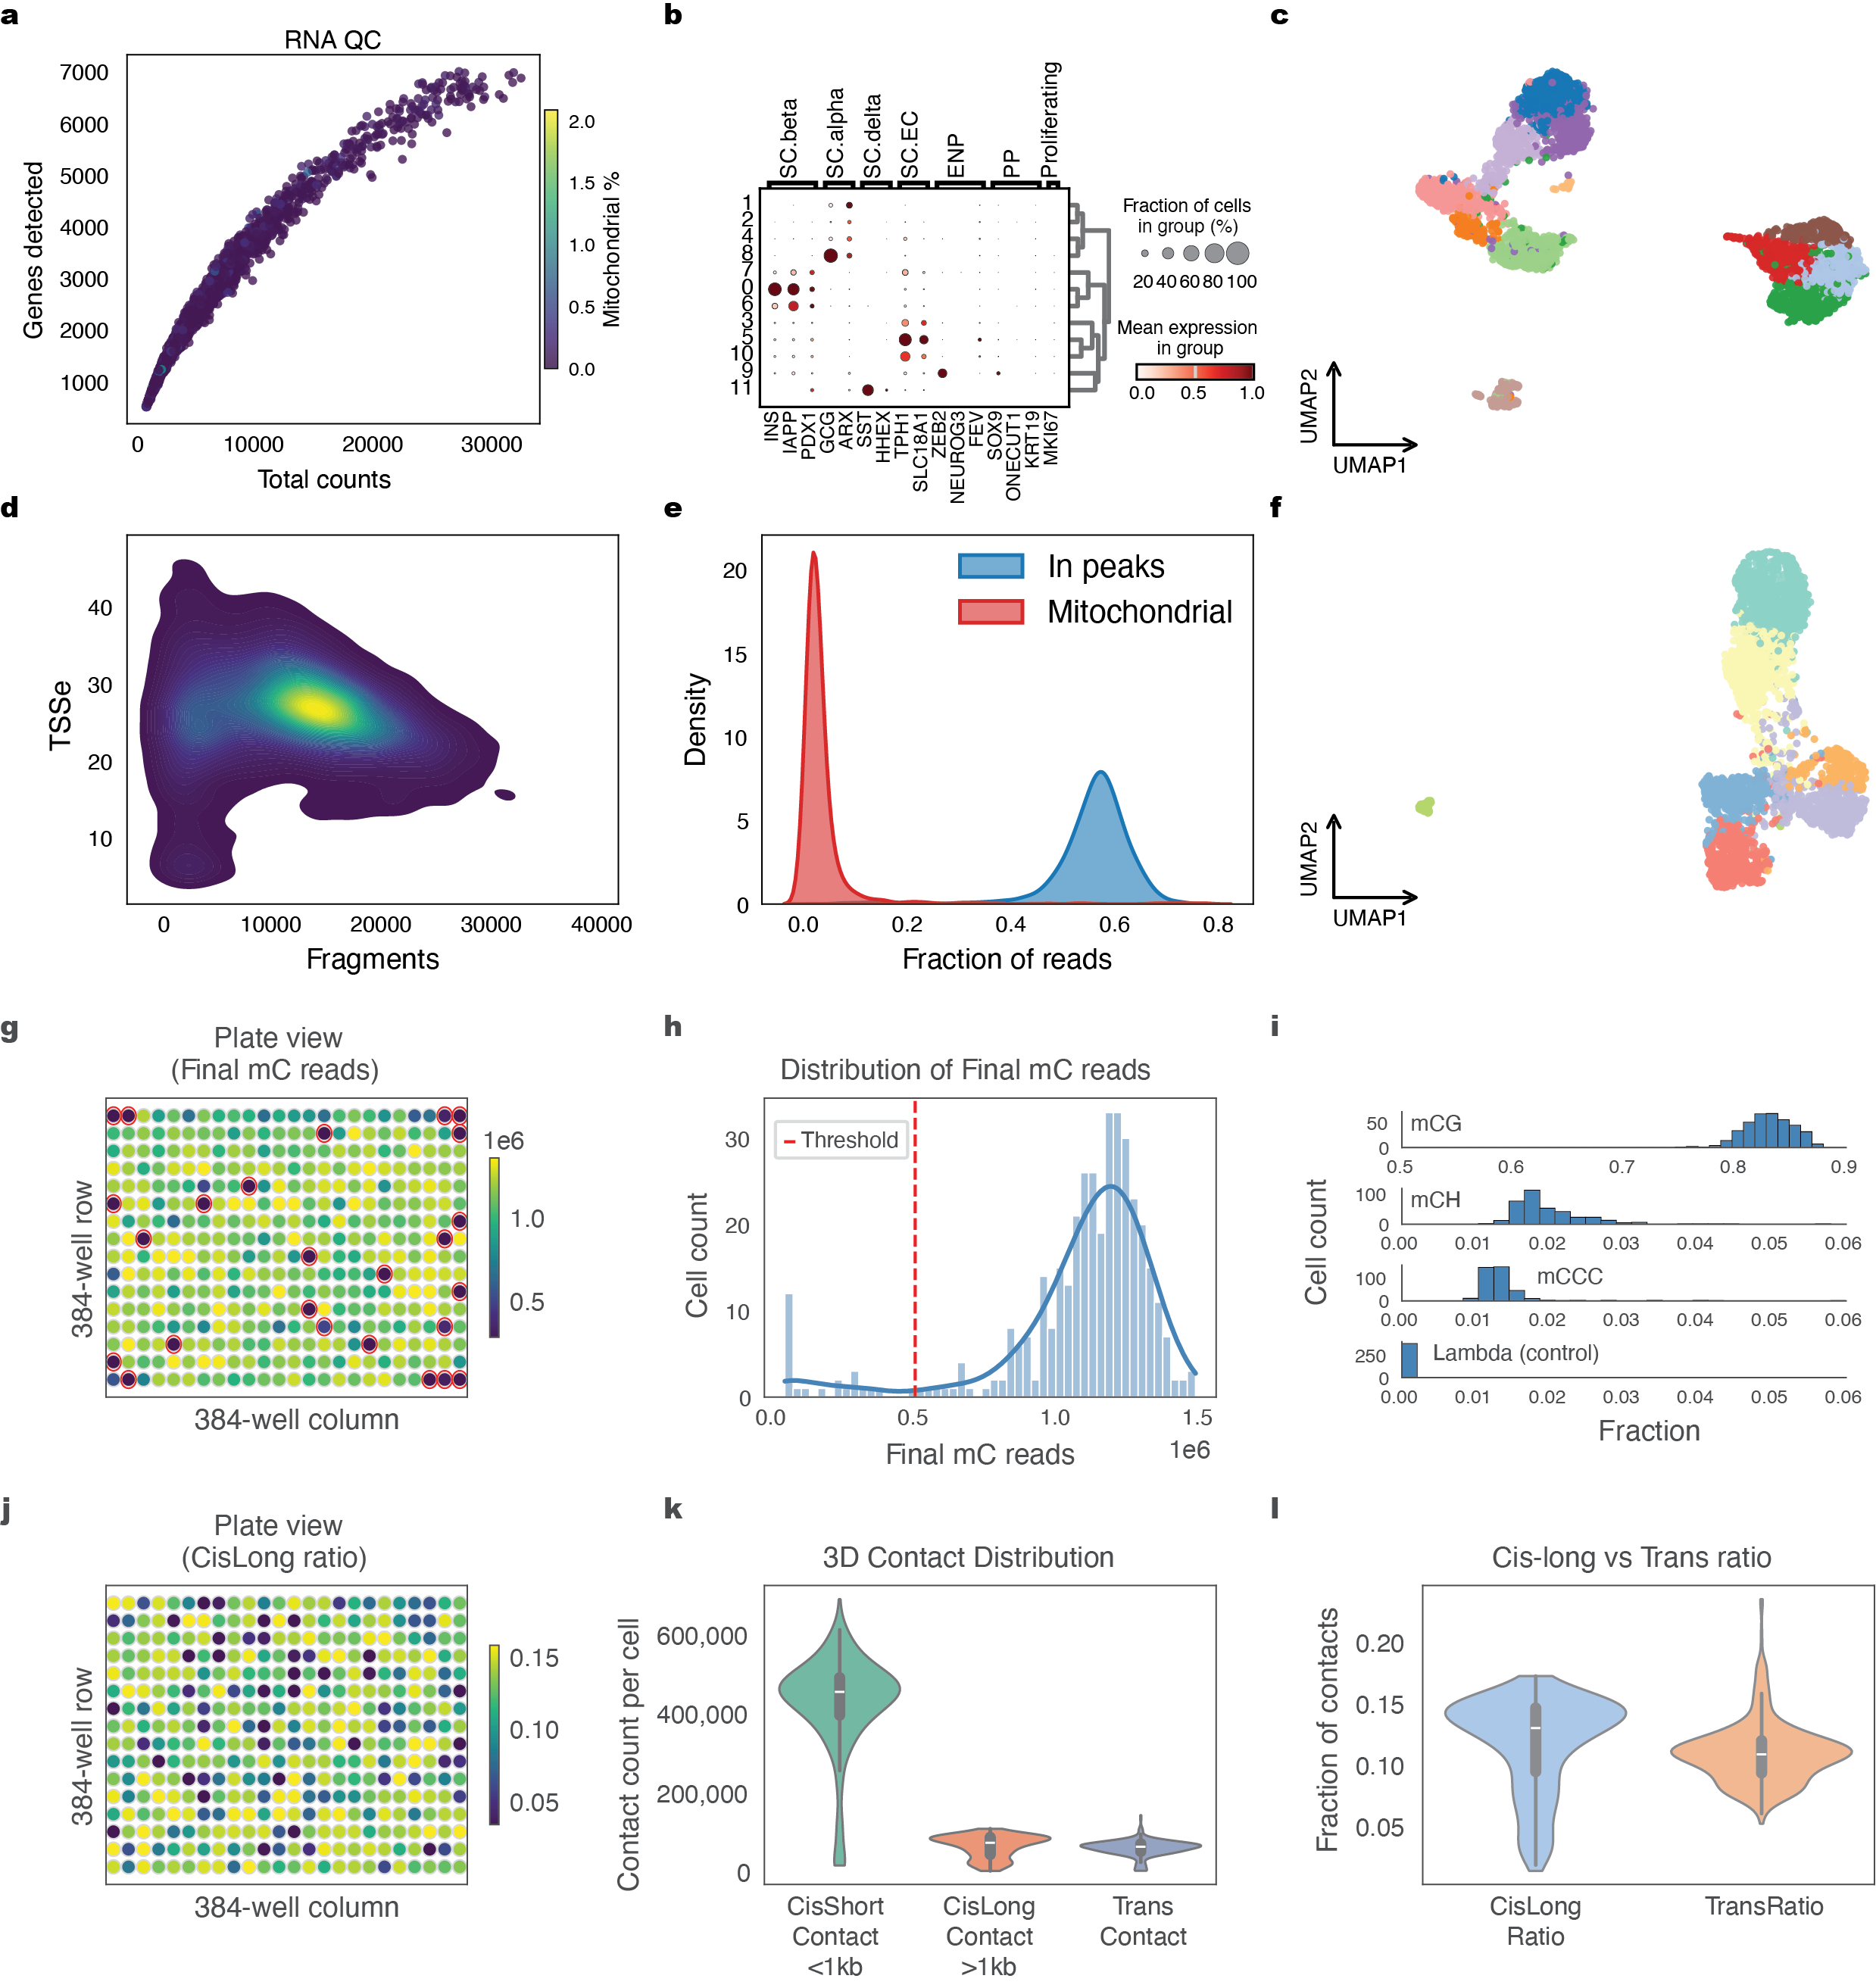
\includegraphics[width=\textwidth]{3_figures-and-files/ExtendedFig1.png}
    \caption[Quality control across molecular modalities]{\textbf{Quality control metrics across molecular modalities for a representative sample (15-1, control, 6 hr)}. \textbf{a}, RNA QC scatterplot showing total UMI counts versus number of genes detected per cell, colored by mitochondrial read percentage. \textbf{b}, Dot plot of marker gene expression across Leiden clusters. \textbf{c}, UMAP embedding of RNA-seq data colored by Leiden clusters. \textbf{d}, ATAC QC density plot of TSS enrichment versus number of fragments per cell. \textbf{e}, Distribution of fraction of reads mapping to peaks (blue) and mitochondrial genome (red) for ATAC data. \textbf{f}, UMAP embedding of ATAC-seq data colored by Leiden clusters. \textbf{g}, Plate layout showing the number of final methylation (mC) reads per well. \textbf{h}, Histogram of final mC read counts per cell, with dashed line indicating threshold for filtering. \textbf{i}, Histogram of global methylation metrics (mCG, mCH, and $\lambda$ spike-in control). \textbf{j}, Plate layout showing cis-long contact ratio per well for 3C data. \textbf{k}, Violin plots of total 3D chromatin contacts per cell, stratified into cis-short (<1 kb), cis-long (>1 kb), and trans interactions. \textbf{l}, Distribution of cis-long versus trans contact ratios per cell.}
    \label{fig:3 supplementary_1}
\end{figure}

\begin{figure}[p]
    \centering
    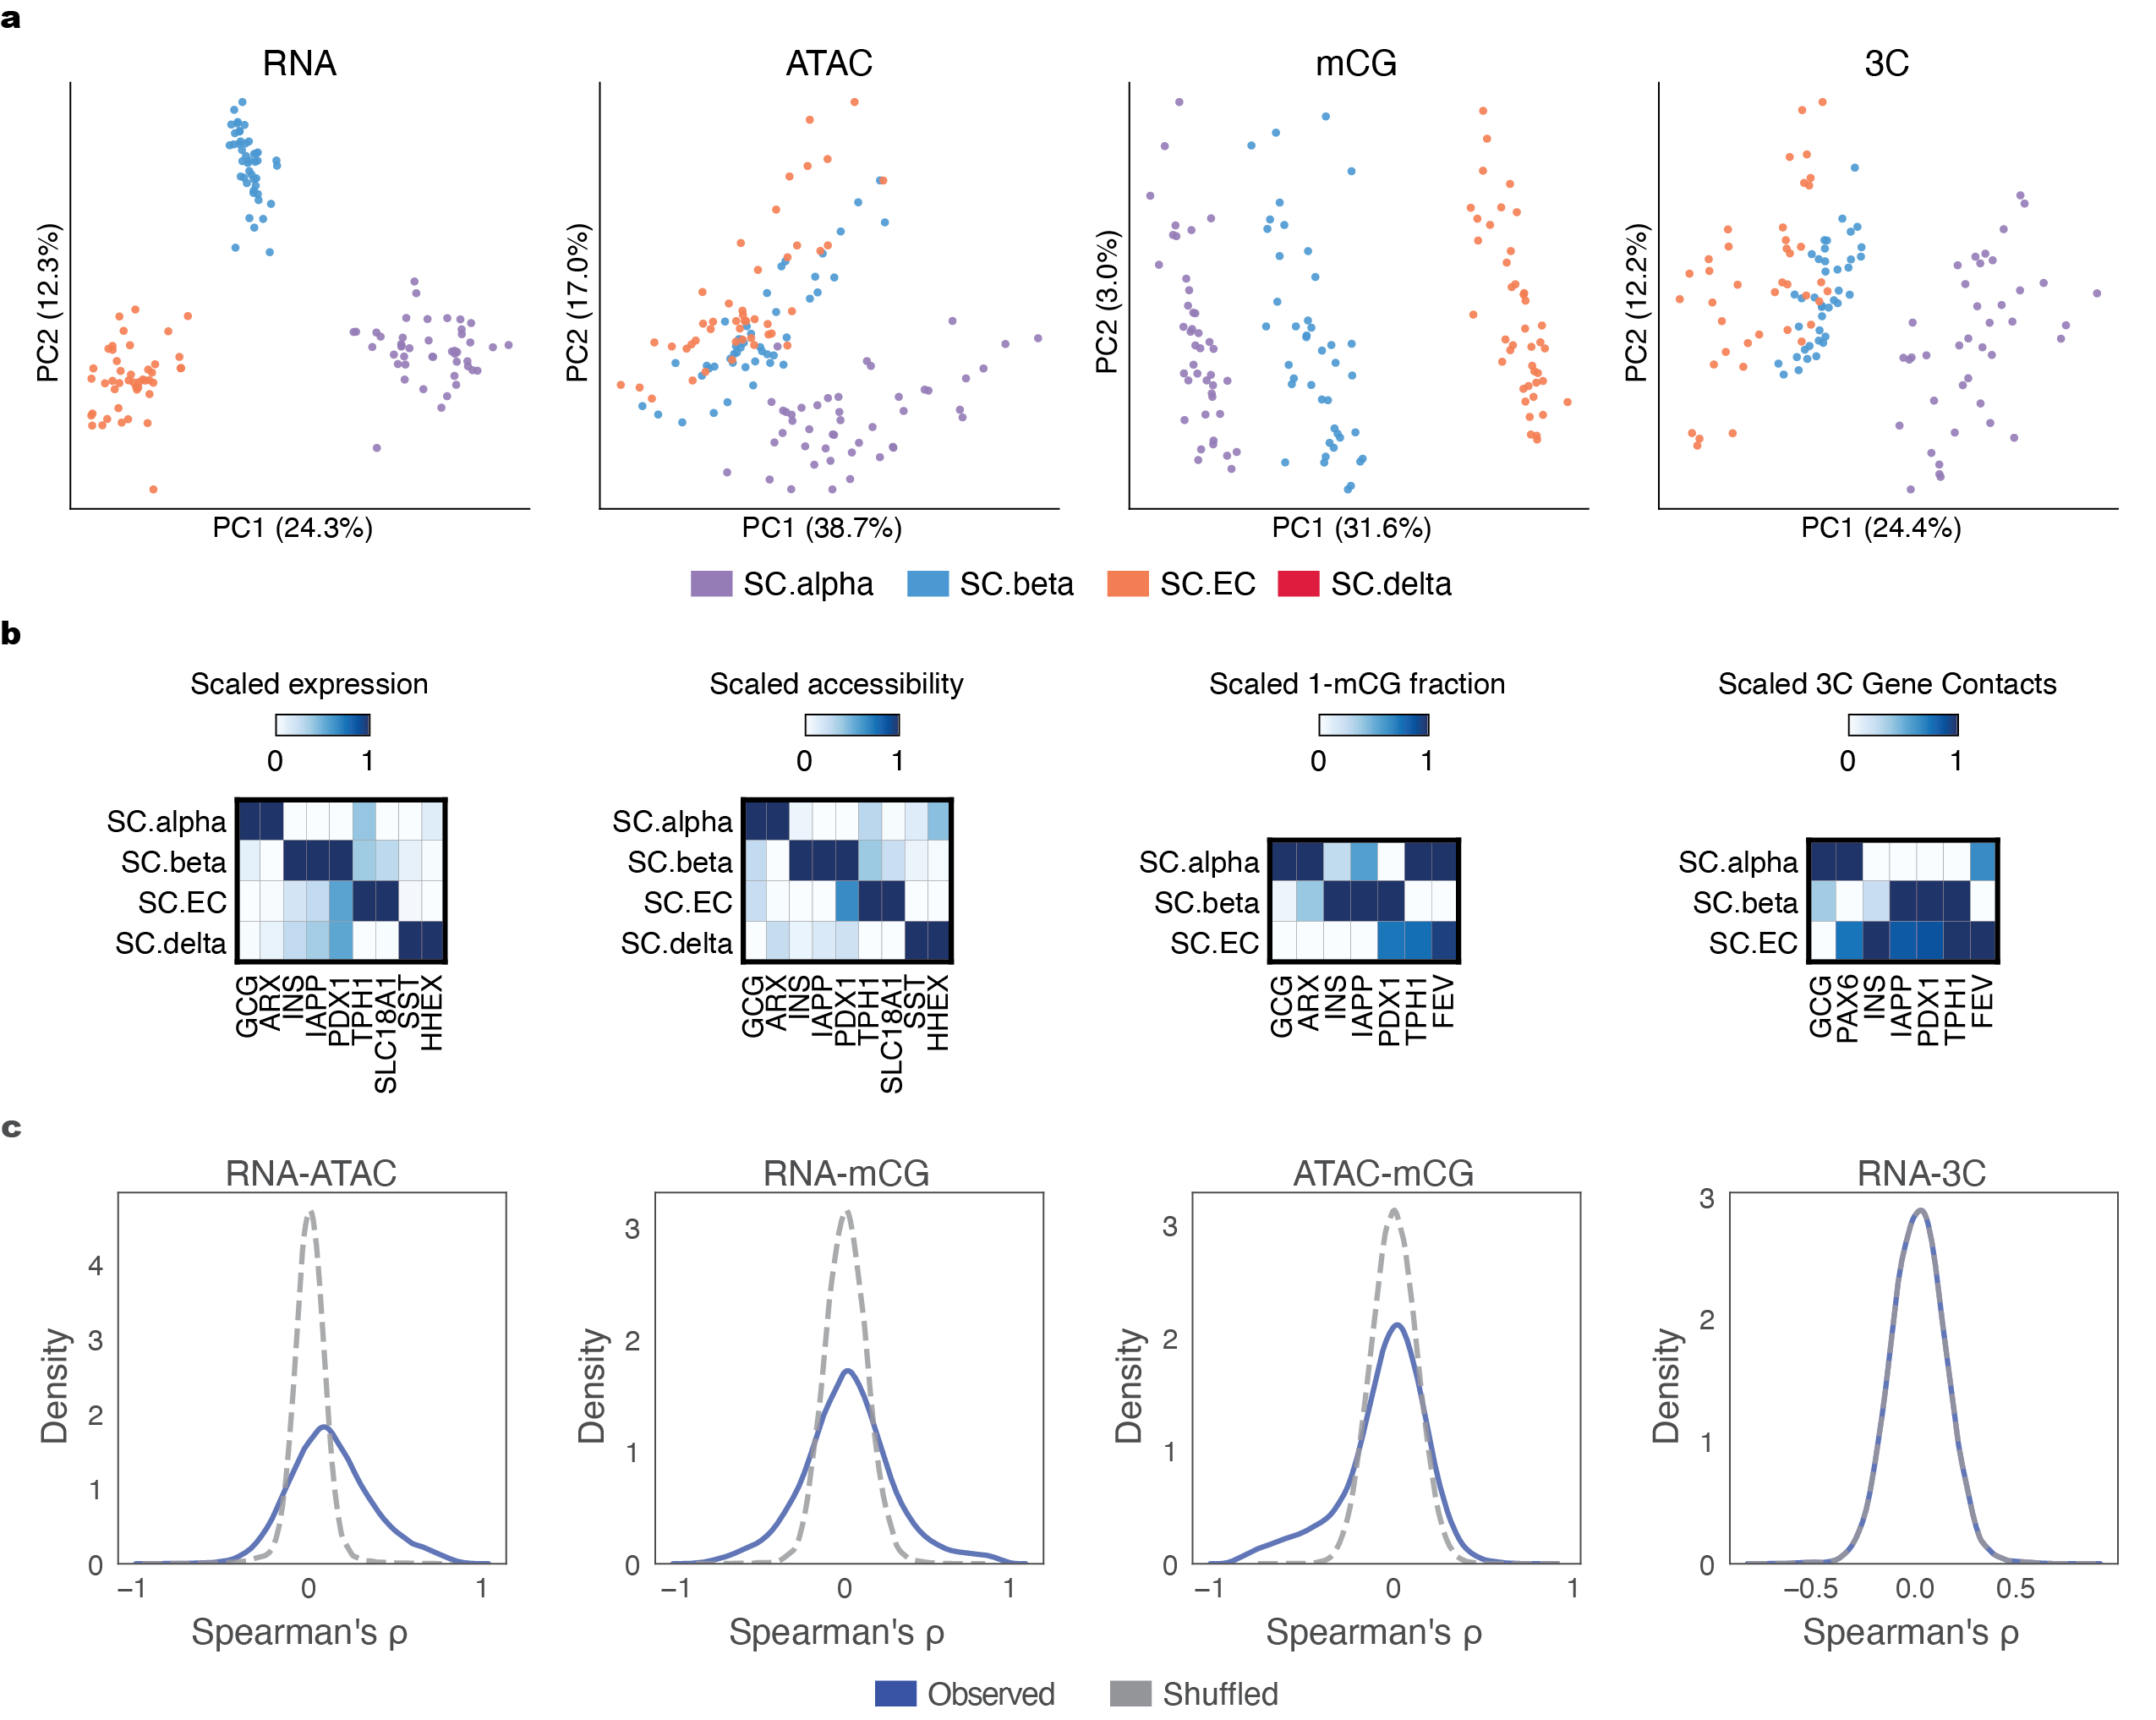
\includegraphics[width=\textwidth]{3_figures-and-files/ExtendedFig2.png}
    \caption[Modality comparison of pseudobulked profiles]{\textbf{Modality comparison of pseudobulked molecular profiles in SC-islet organoids}. \textbf{a}, Principal component analysis of pseudobulk profiles for each cell type across four molecular modalities: mRNA expression (RNA), chromatin accessibility (ATAC), DNA methylation (mCG), and 3D chromatin contacts (3C). Percentage of variance explained are annotated on axes. Points are colored by cell type. \textbf{b}, Heatmaps showing scaled expression, accessibility, methylation, and 3C contact signals across selected marker genes, stratified by cell type. \textbf{c}, Distributions of pairwise Spearman correlations between molecular modalities across genes (blue: observed; gray: shuffled null distribution).}
    \label{fig:3 supplementary_2}
\end{figure}

\begin{figure}[p]
    \centering
    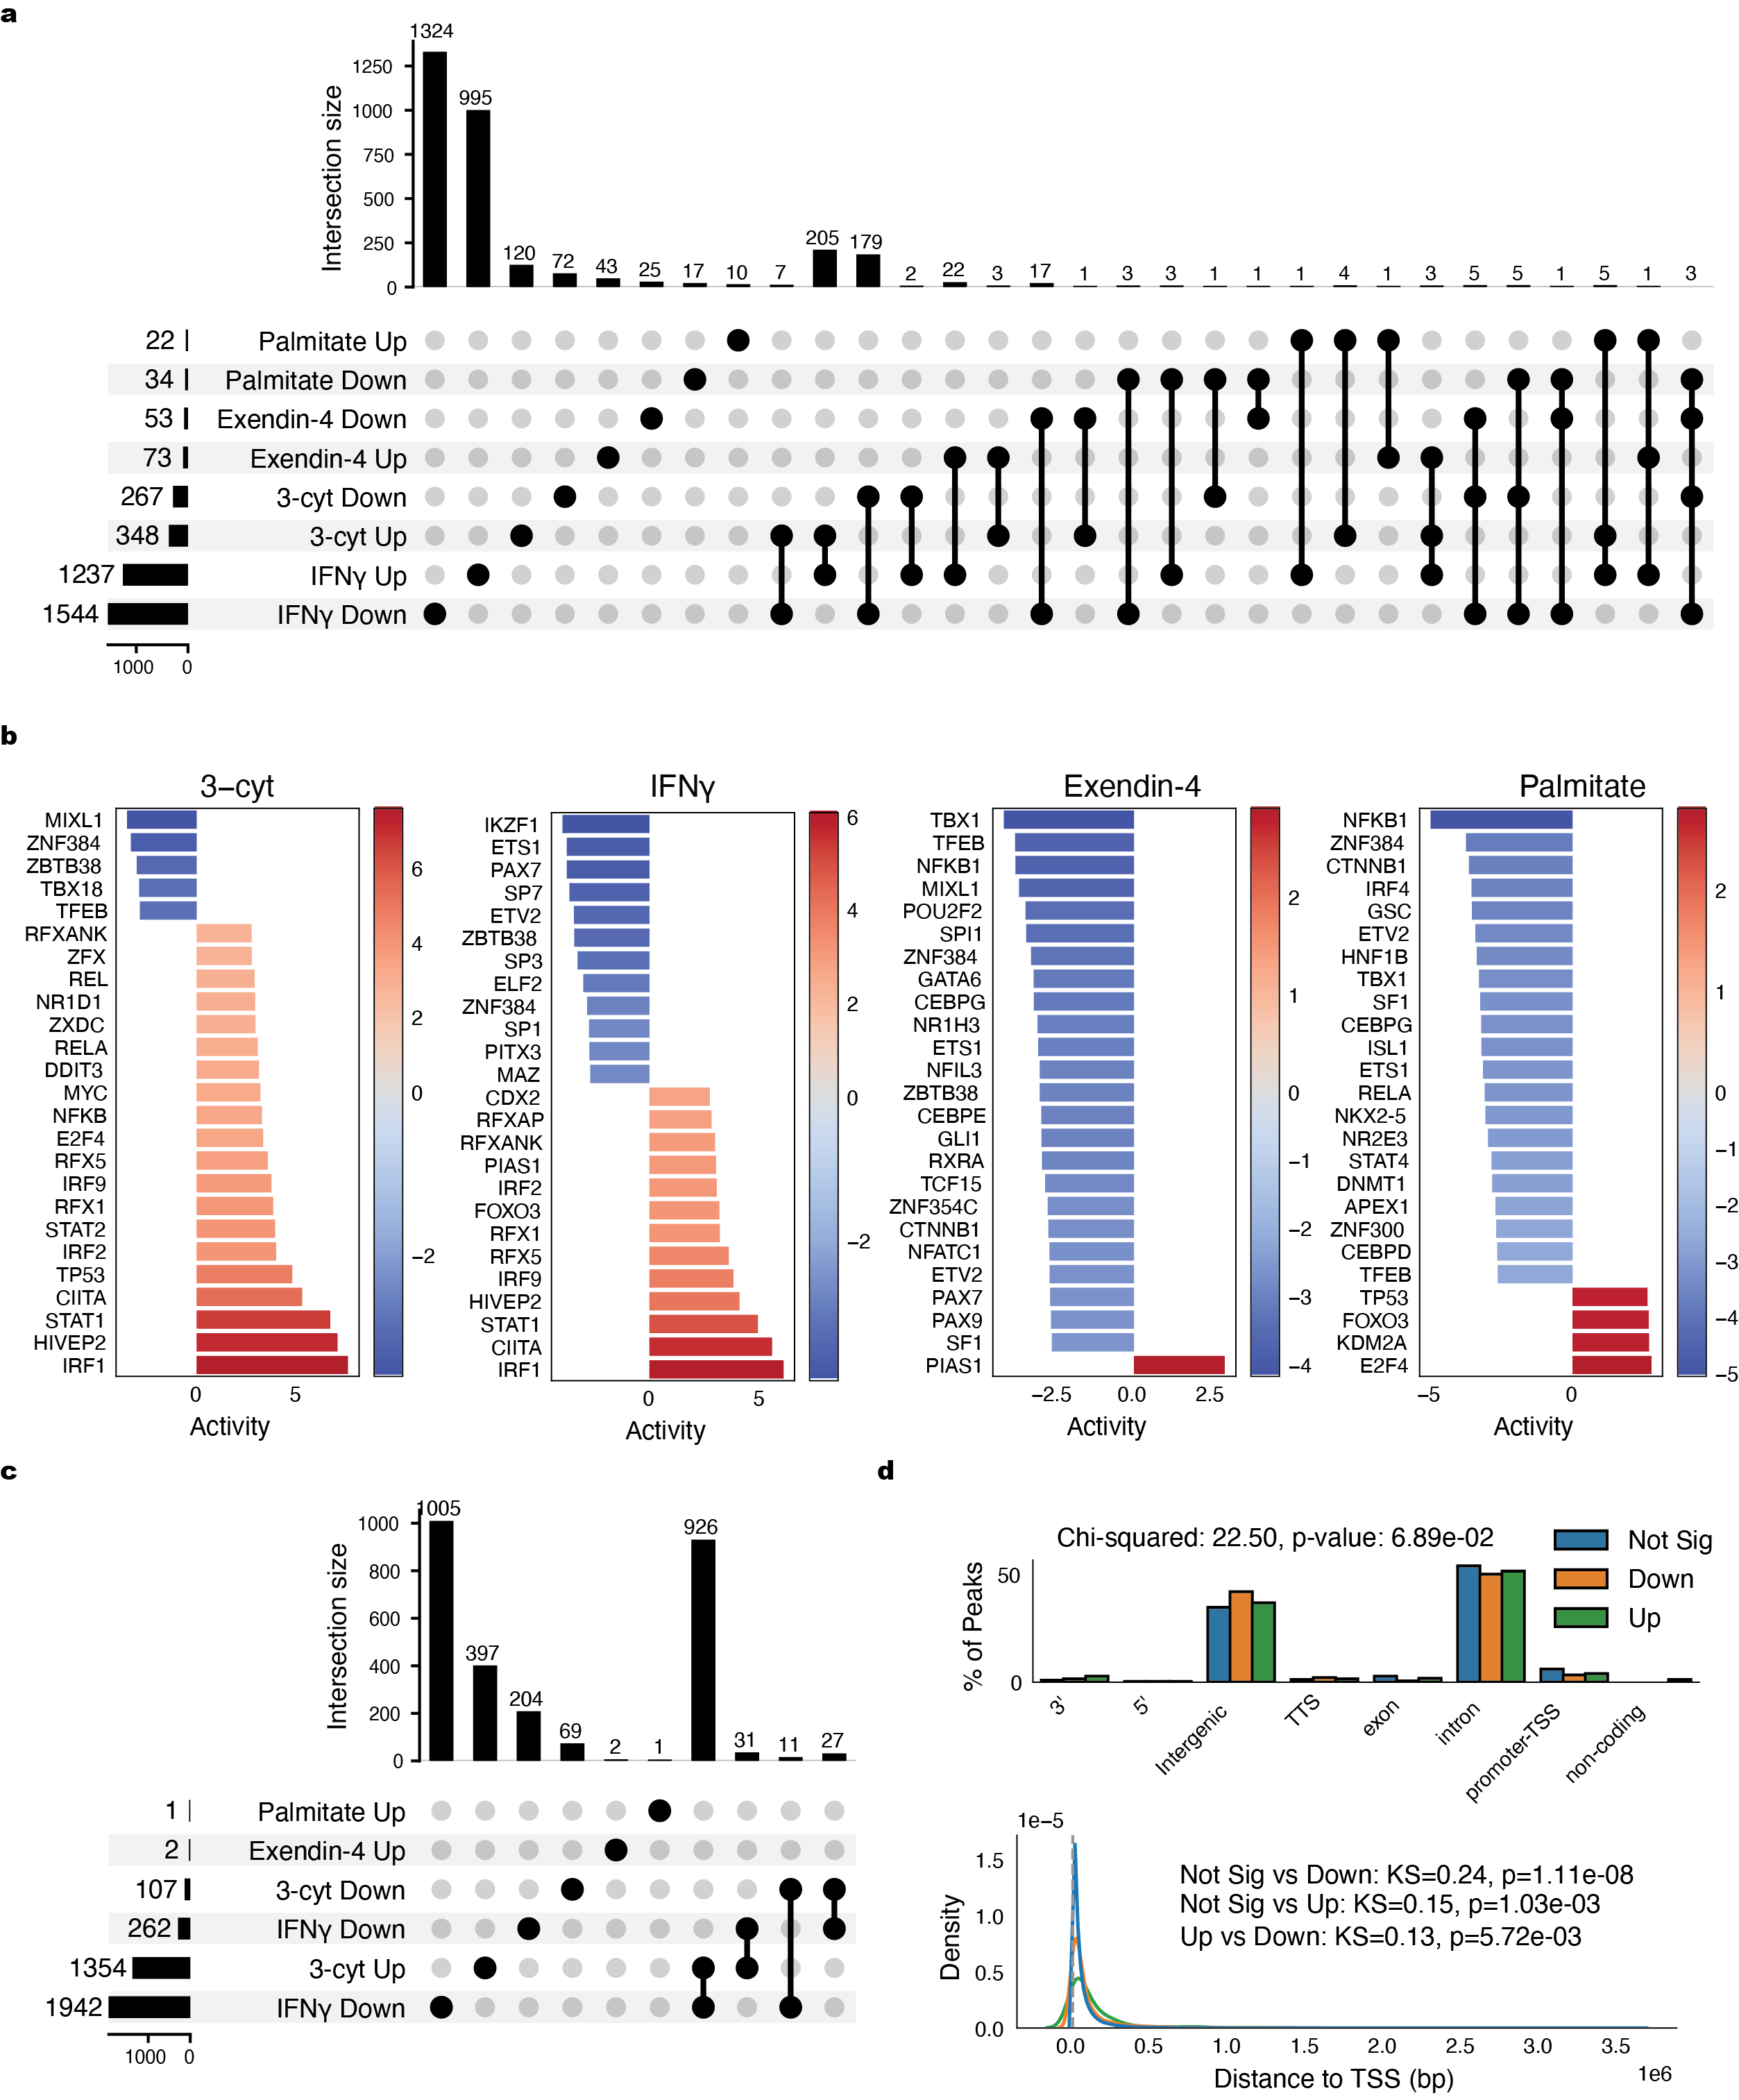
\includegraphics[width=\textwidth]{3_figures-and-files/ExtendedFig3.png}
    \caption[Stimulus-specific and shared SC-beta cell responses]{\textbf{Stimulus-specific and shared multiome responses in SC-beta cells}. \textbf{a}, UpSet plot summarizing the overlap of differentially expressed gene (DEG) sets across treatment conditions. Bars show the number of DEGs (FDR < 0.05 for cytokines, < 0.25 for others) up- or down-regulated in each condition and their intersections. The largest overlaps are observed between cytokine treatments (3-cyt, IFNg), with minimal overlap across non-inflammatory stimuli. \textbf{b}, Inferred transcription factor activity across conditions using decoupleR. \textbf{c}, UpSet plot of DARs stratified by direction of regulation. \textbf{d}, Genomic annotation (top) and TSS-distance distribution (bottom) for DARs. Chi-square p-value is indicated. Pairwise Kolmogorov–Smirnov test statistics and p-values are annotated.}
    \label{fig:3 supplementary_3}
\end{figure}
